\documentclass[pdf,9pt,xcolor=dvipsnames,hide notes]{beamer}
\usetheme{Rochester}
%\usecolortheme{beaver}
\usepackage{verbatim}
\usefonttheme{serif}     % Font theme: serif
\usepackage{ccfonts}     % Font family: Concrete Math
\usepackage[T1]{fontenc}
\usepackage{lmodern}
\usepackage{caption}
\usepackage[caption=false]{subfig}
\usepackage{tabularx}
\usepackage{booktabs}
\usepackage{pdfpages}
\usepackage{graphicx} 
\usepackage{hyperref}
\DeclareCaptionLabelSeparator{horse}{:\quad} % change according to your needs
\captionsetup{
  labelsep = horse,
  figureposition = bottom % proper spacing between figure and caption
}
\usepackage{graphicx,amsfonts,booktabs,hyperref,subfig,amssymb,amsmath,amsthm,tabularx,multirow,enumerate}
%\usepackage{parskip}
%\setlength{\parindent}{10pt}
\usepackage{ragged2e,tikz,color,colortbl,xcolor}

\DeclareMathOperator{\Ima}{Im}

% Real Number
\newtheorem{proposition}{Proposition}
\newcommand{\R}{\mathbb R}
% natural numbers
\newcommand{\Nat}{\mathbb N}
% complex numbers
\newcommand{\C}{\mathbb C}
\newcommand{\E}{\mathbb{E}}
\newcommand{\Var}{\mathrm{Var}}
\newcommand{\Cov}{\mathrm{Cov}}
\newcommand{\Corr}{\mathrm{Corr}}
\newcommand{\Expect}{{\rm I\kern-.3em E}}
\setbeamertemplate{theorems}[numbered]

\setbeamertemplate{caption}[numbered]
\setbeamercolor{postit}{use=structure,fg=black,bg=structure!13!white}
\newcommand{\otoprule}{\midrule[\heavyrulewidth]}
\makeatletter
    \newenvironment{withoutheadline}{
        \setbeamertemplate{headline}[default]
        \def\beamer@entrycode{\vspace*{-\headheight}}
    }{}
\makeatother
\title[PPGE/UFRGS]{Worst Case CVaR Portolio Optimization with Multidimensional Copulas}
%\subtitle{}
\author[Fernando A. Boeira Sabino da Silva]{Fernando A. Boeira Sabino da Silva\inst{1}}
\author[Flavio A. Ziegelmann]{Fernando A. Boeira Sabino da Silva\inst{1,2}, Flavio A. Ziegelmann\inst{1,2}}
\author[Cristina Tessari]{Fernando A. Boeira Sabino da Silva\inst{1}, Flavio A. Ziegelmann\inst{1,2}, Cristina Tessari\inst{3}}
\institute[Department of Statistics/UFRGS, PPGE/UFRGS,Finance Division/Columbia Business School]{\inst{1} Department of Statistics/UFRGS, \inst{2} PPGE/UFRGS, \inst{3} Finance Division/Columbia Business School}
%\date{\today} % (optional)
\date{} % (optional)

\hypersetup{
    pdftitle={TITLE},
    pdfauthor={AUTHOR},
    pdfsubject={SUBJECT},
    pdfkeywords={KEYWORD} {KEYWORD} {KEYWORD},
    colorlinks=true,
    linkcolor=blue,
    citecolor=blue,
    filecolor=magenta,
    urlcolor=blue
    }
\usepackage{threeparttable}


\begin{document}
\justifying

\frame{\titlepage}

%\frame{\frametitle{Table of contents}\tableofcontents}

\section{Introduction}

\begin{frame}[label=frame1]
\frametitle{Introduction and Motivation}

\begin{itemize}
\justifying

\item The seminal article \emph{Portfolio Selection} published by Harry Markowitz (1952) introduces the foundation for modern portfolio theory (MPT) or mean-variance analysis.

\vspace{0.3cm}

\item Markowitz considered the problem of an agent who wishes to find the maximum (expected)
return for a given level of risk or minimize risk for a given level of
return.

\vspace{0.3cm}

\item  By diversifying a portfolio among investments
that have different return patterns, investors can build such an efficient
portfolio.
%, i.e., an optimized portfolio that dominate all other feasible
%portfolios in terms of their risk-return trade-off. 

\end{itemize}
%\begin{flushright}
%\hyperlink{counterexample}{\beamerreturnbutton{Counterexample}}
%\end{flushright}

\end{frame}

\begin{frame}[label=frame1d]
	\frametitle{Introduction and Motivation}
	
	\begin{itemize}
		\justifying
		
		%		\item The original Markowitz model finds a set of "optimal" portfolio weights given
		%		a set of expected returns and covariances. 
		
		\vspace{0.3cm}
		
		\item A well-known problem of
		the Markowitz model is its sensitivity to the input parameters. 
		
		\vspace{0.3cm}
		
%		\item In practice, the implementation of strategies based on the risk-return trade-off remains a fundamental challenge in many areas of financial management, since it is necessary to obtain accurate estimates of the expected returns of the assets and the covariance matrix of these returns.
		
		\item In practice, the implementation of strategies based on the risk-return trade-off remains a fundamental challenge in many areas of financial management, since estimation errors of the expected returns of the assets and the covariance
		matrix of these returns can significantly affect cause an impact in the asset allocations weights, no
		longer leading to an efficient portfolio.
		
		%		the outcome of the
%		optimization problem.
		
	
		\vspace{0.3cm}
		
	\item This issue can be overcome by employing robust optimization and
	worst case techniques (\textcolor{blue}{Zhu and Fukushima}, \textcolor{blue}{2009}) in which assumptions about the
	distribution of the random variable are relaxed, and thus, we obtain the
	optimal portfolio solution by optimizing over a prescribed feasible set and
	possible densities.
		
	\end{itemize}
	%\begin{flushright}
	%\hyperlink{counterexample}{\beamerreturnbutton{Counterexample}}
	%\end{flushright}
	
	
\end{frame}

\begin{frame}[label=frame1d]
	\frametitle{Introduction and Motivation}
	
	\begin{itemize}
		\justifying
		
		\item Akin to
				the classical Markowitz portfolio, in this approach we want to determine
				the weights that maximize the portfolio return for a specified VaR or CVaR
				at a given confidence level or minimize these quantiles for a given
				confidence level subject to a fixed portfolio return.
				
				\vspace{0.3cm}
				
				\item  \textcolor{blue}{Artzner \emph{et al}}., \textcolor{blue}{1999} show that VaR has undesirable properties such as lack
				of sub-additivity and thus it is not a coherent measure.
		
			\end{itemize}
	
\end{frame}

\begin{frame}[label=frame1b]
	\frametitle{Introduction and Motivation}
	
	\begin{itemize}
		\justifying
		
\vspace{0.3cm}

%\item \textcolor{blue}{Uryasev and Rockafellar}, \textcolor{blue}{2001} show that VaR may be a non-convex function with respect to
%portfolio weights, which can yield to multiple portfolio local solutions,
%but CVaR is coherent both for continuous and discrete distributions and it
%is a convex function. 
%
%\vspace{0.3cm}

	\item \textcolor{blue}{Uryasev and Rockafellar}, \textcolor{blue}{2001} show that an outright optimization with respect to CVaR is numerically difficult due to the dependence of the
CVaR on VaR. 

\vspace{0.3cm}

	\item However, \textcolor{blue}{Rockafellar and Uryasev}, \textcolor{blue}{2000} show that VaR and CVaR can be	computed simultaneously, introducing auxiliary risk measures. 
	
	\vspace{0.3cm}
	
	\item Their approach can be
	used in conjunction with scenario based optimization algorithms reducing the
	problem to a linear programming problem which allows us to optimize a portfolio with very large dimensions and stable numerical implementations.
	
	\vspace{0.3cm}
	
	\item \textcolor{blue}{Kakouris and Rustem}, \textcolor{blue}{2014} show how copula-based models can be
	introduced in the Worst Case CVaR framework. This approach is
	motivated by an investor's desire to be protected against the worst possible
	scenario.

	
    \end{itemize}
	%\begin{flushright}
	%\hyperlink{counterexample}{\beamerreturnbutton{Counterexample}}
	%\end{flushright}
	
\end{frame}

\begin{frame}[label=frame2]
\frametitle{Goals}

\begin{enumerate}[(1)]
\justifying

\item Evaluate the out-of-sample performance of the Worst Case Copula-CVaR and compare it to benchmark approaches in the long term in terms of wealth accumulation and
downside risk.

\vspace{0.3cm}

\item Select a diversified set of assets that can be
useful during crises and tranquil periods, i.e., that somehow involves hedging of decisions
to protect the investors against any market conditions.

\end{enumerate}

\end{frame}

\section{Conditional Value-at-Risk}
\begin{frame}[label=frame2b2]
	\frametitle{Conditional Value-at-Risk}
	\begin{itemize}
		\justifying
		
		\item 	Let $Y$ be a stochastic vector standing for market uncertainties and $F_{Y}$
		be its distribution function, i.e., $F_{Y}\left( u\right) =P\left( Y\leq
		u\right) $. Let also $F_{Y}^{-1}\left( v\right) =\inf \left\{ u:F_{Y}\left(
		u\right) \geq v\right\} $ be its right continuous inverse and assume that it
		has a probability density function represented by $p(y)$. Define the $VaR_{\beta
		}$\thinspace\ as the $\beta $-quantile by
		\begin{eqnarray}
		VaR_{\beta }\left( Y\right) &=& \arg \min \left\{ \alpha \in
		\mathbb{R}
		:P\left( Y\leq \alpha \right) \geq \beta \right\}  \label{one} \\
		&=&F_{Y}^{-1}\left( \beta \right) \text{,}  \notag
		\end{eqnarray}%
		and the $CVaR_{\beta }$ as the solution to the following optimization
		problem:
		\begin{equation}
		CVaR_{\beta }\left( Y\right) =\inf \left\{ \alpha \in
		\mathbb{R}
		:\alpha +\frac{1}{1-\beta }E\left[ Y-\alpha \right] ^{+}\right\} \text{,}
		\label{two}
		\end{equation}%
		where $\left[ t\right] ^{+}=\max \left( t,0\right) $.
		
	\end{itemize}
	%\begin{flushright}
	%\hyperlink{counterexample}{\beamerreturnbutton{Counterexample}}
	%\end{flushright}
	
\end{frame}

\begin{frame}[label=frame2b3]
	\frametitle{Conditional Value-at-Risk}
	\begin{itemize}
		\justifying
		
		\item \textcolor{blue}{Uryasev and Rockafellar}, \textcolor{blue}{1999} have shown that the $CVaR$ is the conditional
		expectation of $Y$, given that $Y\geq VaR_{\beta }$, i.e.,
		\begin{equation}
		CVaR_{\beta }\left( Y\right) =\mathbb{E}\left( Y\left\vert Y\geq VaR_{\beta
		}\left( Y\right) \right. \right) .  \label{three}
		\end{equation}
		
		\vspace{0.3cm}
		
		\item Let $f\left( x,y\right) $ be a loss function depending upon a decision
		vector $x$ that belongs to any arbitrarily chosen subset $X\in
		%BeginExpansion
		\mathbb{R}
		%EndExpansion
		^{n}$ and a random vector $y\in
		%BeginExpansion
		\mathbb{R}
		%EndExpansion
		^{m}$. 
		
			\vspace{0.3cm}
		
		\item In a portfolio optimization problem, the decision vector $x$ can be a
		vector of portfolios' weights, $X$ be a set of feasible portfolios,
		subject to linear constraints and $y$ a vector that stands for market variables that can affect the loss.
		
	\end{itemize}
	%\begin{flushright}
	%\hyperlink{counterexample}{\beamerreturnbutton{Counterexample}}
	%\end{flushright}
	
\end{frame}



\begin{frame}[label=frame2b5]
	\frametitle{Conditional Value-at-Risk}
	\begin{itemize}
		\justifying
		
		\item Using $\left( \ref{three}\right) $ we can
		write the $CVaR$ function, at confidence level $\beta $, by%
		\begin{equation}
		CVaR_{\beta }\left( x\right) = \frac{1}{1-\beta }\int_{f(x,y)\geq VaR_{\beta
			}\left( x\right) }f(x,y)p(y)dy\text{,}  \label{five}
		\end{equation}
		
		\vspace{0.3cm}
		
		\item The optimization of $CVaR$ is difficult because of the presence of the $VaR$
		in its definition (it requires the use of the nonlinear function max). 
		
		\vspace{0.3cm}
		
		\item The main contribution of \textcolor{blue}{Rockafellar and Uryasev}, \textcolor{blue}{2000} was to define a simpler auxiliary function
		\begin{equation}
		F_{\beta }\left( x,\alpha \right) = \alpha +\frac{1}{1-\beta }%
		\int_{f(x,y)\geq \alpha }\left( f(x,y)-\alpha \right) p(y)dy\text{,}
		\label{six}
		\end{equation}%
		which can be used instead of $CVaR$ directly, without need to compute $VaR$
		first due to the following proposition (see \textcolor{blue}{Pflug}, \textcolor{blue}{2000}):
		
		\vspace{0.3cm}
		
					
			
	\end{itemize}
	%\begin{flushright}
	%\hyperlink{counterexample}{\beamerreturnbutton{Counterexample}}
	%\end{flushright}
	
\end{frame}

\begin{frame}[label=frame2b6]
	\frametitle{Conditional Value-at-Risk}
	
	\begin{proposition}
			The function $F_{\beta }\left( x,\alpha \right) $ is convex with respect to $%
			\alpha $. In addition, minimizing $F_{\beta }\left( x,\alpha \right) $ with
			respect to $\alpha $ gives $CVaR$ and $VaR$ is a minimum point of this
			function with respect to $\alpha $, i.e.
			\begin{equation}
			\underset{\alpha \in
				%BeginExpansion
				\mathbb{R}
				%EndExpansion
			}{\min }~F_{\beta }\left( x,\alpha \right) =F_{\beta }\left( x,VaR_{\beta
			}\left( x\right) \right) =CVaR_{\beta }(x)  \label{seven}
			\end{equation}
		\end{proposition}
		
		\vspace{0.3cm}
		
			\begin{itemize}
			\justifying
			
					\item Moreover, we can use $F_{\beta }\left( x,\alpha \right) $ to find the optimal weights, $CVaR$ and
			$VaR$ simultaneously over an allowable feasible set, i.e.,
			\begin{equation}
			\underset{x\in X}{\min }~CVaR_{\beta }(x)=\underset{}{\underset{\left(
					x,\alpha \right) \in X\times
					%BeginExpansion
					\mathbb{R}
					%EndExpansion
				}{\min }F_{\beta }\left( x,\alpha \right) }.  \label{eight}
			\end{equation}
			
			\vspace{0.3cm}
			
			\item \textcolor{blue}{Pflug}, \textcolor{blue}{2000} show that under quite general conditions $F_{\beta
			}\left( x,\alpha \right) $ is a smooth function. In addition, if $f(x,y)$ is
			convex with respect to $x$, then $F_{\beta }\left( x,\alpha \right) $ is
			also convex with respect to $x$. 
			
			\vspace{0.3cm}
			
			\item Hence, if the allowable set $X$ is also
			convex, we then have to solve a smooth convex optimization problem.
			
		\end{itemize}
	%\begin{flushright}
	%\hyperlink{counterexample}{\beamerreturnbutton{Counterexample}}
	%\end{flushright}
	
\end{frame}

\subsection{CVaR Minimization with Finite Number of Scenarios}
\begin{frame}[label=frame2b7]
	\frametitle{Optimization Problem}
	
		\begin{itemize}
		\justifying
		
		\item Assume that the analytical representation for the density $p(y)$ is not
		available, but we can approximate $F_{\beta }\left( x,\alpha \right) $ using
		$J$ scenarios, $y_{j}$, $j=1,...,J$ which are sampled from the density
		function $p(y)$. 
		
		\vspace{0.3cm}
		
		\item We approximate
		\begin{eqnarray}
		F_{\beta }\left( x,\alpha \right) &=&\alpha +\frac{1}{1-\beta }%
		\int_{f(x,y)\geq \alpha }\left( f(x,y)-\alpha \right) p(y)dy  \notag \\
		&=&\alpha +\frac{1}{1-\beta }\int_{y\in
			%BeginExpansion
			\mathbb{R}
			%EndExpansion
			^{m}}\left( f(x,y)-\alpha \right) ^{+}p(y)dy  \label{fb}
		\end{eqnarray}%
		by its discretized version
		\begin{equation*}
		\widetilde{F}_{\beta }\left( x,\alpha \right) =\alpha +\frac{1}{\left(
			1-\beta \right) J}\sum_{j=1}^{J}\left( f(x,y_{j})-\alpha \right) ^{+}.
		\end{equation*}%
				
	\end{itemize}
	%\begin{flushright}
	%\hyperlink{counterexample}{\beamerreturnbutton{Counterexample}}
	%\end{flushright}
	
\end{frame}

\begin{frame}[label=frame2b8]
	\frametitle{Optimization Problem}
	
	\begin{itemize}
		\justifying
		
		\item Assuming that the feasible set $X$ and the loss
		function $f(x,y_{j})$ are convex, we solve the following convex optimization problem:
		\begin{equation}
		\underset{x\in X,\alpha \in
			%TCIMACRO{\U{211d} }%
			%BeginExpansion
			\mathbb{R}
			%EndExpansion
		}{\min }\widetilde{F}_{\beta }\left( x,\alpha \right) .  \label{ten}
		\end{equation}
		
		\vspace{0.3cm}
		
		\item In addition, if the loss function $f(x,y)$ is linear with respect to
		\thinspace $x$, then the optimization problem $\left( \ref{ten}\right) $
		reduces to the following linear programming (LP) problem:%
		\begin{equation}
		\underset{x\in
			%TCIMACRO{\U{211d} }%
			%BeginExpansion
			\mathbb{R}
			%EndExpansion
			^{n},z\in
			%TCIMACRO{\U{211d} }%
			%BeginExpansion
			\mathbb{R}
			%EndExpansion
			^{J},\alpha \in
			%TCIMACRO{\U{211d} }%
			%BeginExpansion
			\mathbb{R}
			%EndExpansion
		}{\min }\alpha +\frac{1}{\left( 1-\beta \right) J}\sum_{j=1}^{J}z_{j}
		\label{eleven}
		\end{equation}%
		\begin{equation}
		subject\text{ } to\text{ }x\in X,  \label{12}
		\end{equation}
		\begin{equation}
		z_{j}\geq f(x,y_{j})-\alpha ,\text{ }z_{j}\geq 0,\text{ }j=1,...,J,
		\label{13}
		\end{equation}
		where $z_{j}$ are indicator variables. 
		
	\end{itemize}
	%\begin{flushright}
	%\hyperlink{counterexample}{\beamerreturnbutton{Counterexample}}
	%\end{flushright}
	
\end{frame}

\begin{frame}[label=frame2b9]
	\frametitle{CVaR Minimization with Finite Number of Scenarios}
	
	\begin{itemize}
		\justifying
		
		\item By solving the LP problem we
		find the optimal decision vector, $x^{\ast }$, the optimal $VaR$, $\alpha
		^{\ast }$, and consequently the optimal $CVaR$, $\widetilde{F}_{\beta
		}\left( x=x^{\ast },\alpha=\alpha ^{\ast }\right) $.
	
	\vspace{0.3cm}
	
	\item Therefore, the optimization problem can be solved using algorithms that are
	capable of solving efficiently very large-scale problems with any
	distribution within reasonable time and high reliability as, for example,
	simplex or interior point methods.
	
		
	\end{itemize}
	%\begin{flushright}
	%\hyperlink{counterexample}{\beamerreturnbutton{Counterexample}}
	%\end{flushright}
	
\end{frame}

\section{The Models}
\subsection{The Worst Case CVaR}

%\begin{frame}[label=frame2c]
%\frametitle{The Worst Case CVaR}
%
%\begin{itemize}
%	\justifying
%	
%	\item Assume that there are $n$ risky assets and denote
%	by $r$ their random (log)returns vector, i.e., $\mathbf{r}\mathbf{=}\left(
%	r_{1},...,r_{n}\right) ^{\top }$, with expected returns $\mathbf{\mu }%
%	\mathbf{=}\left( \mu _{1},...,\mu _{n}\right) ^{\top }$ and covariance
%	matrix $\Sigma _{nxn}$. 
%	
%	\vspace{0.3cm}
%	
%	\item Let also $r_{f}$ represent the risk-free asset
%	returns and the decision (portfolio's weights) vector by $\mathbf{w}\mathbf{=%
%	}\left( w_{1},...,w_{n}\right) ^{\top }$. Also assume that $\mathbf{w}\in
%	\mathcal{W}$, where $\mathcal{W}$ is a feasible set and that the portfolio
%	return loss function $f_{L}\left( \mathbf{w,r}\right) $ is a convex (linear)
%	function given by
%	
%	\begin{equation*}
%	f_{L}(\mathbf{w},\mathbf{r})=\mathbf{w}^{^{\top }}\mathbf{r}\text{.}
%	\end{equation*}
%	
%		\vspace{0.3cm}
%	
%	\item By definition, the portfolio return is the negative of the loss, i.e., $-%
%	\mathbf{w}^{^{\top }}\mathbf{r}$.
%	
%	
%
%	
%\end{itemize}
%
%\end{frame}

\begin{frame}[label=frame2d]
	\frametitle{The Worst Case CVaR}
	
	\begin{itemize}
		\justifying

\item Instead of assuming the precise distribution of the random vector $r$,
\textcolor{blue}{Zhu and Fukushima}, \textcolor{blue}{2009} consider the case where the probability distribution $\pi$
is only known to belong to a certain set, say $\mathcal{P}$, defined the
worst-case CVaR (WCVaR) as the CVaR when the worst-case probability
distribution in the set $\mathcal{P}$ occurs.

\end{itemize}

\begin{definition}
	Given a confidence level $\beta ,$ $\beta \in (0,1),$ the worst-case CVaR
	for fixed $w\in \mathcal{W}$ with respect to the uncertainty set $\mathcal{P}
	$ is defined as
	\begin{eqnarray}
	WCVaR_{\beta }\left( \mathbf{w}\right) &\equiv &\underset{\pi \in \mathcal{P}%
	}{\sup }~ CVaR_{\beta }\left( \mathbf{w}\right)  \notag \\
	&=&\underset{\pi \in \mathcal{P}}{\sup }~\underset{\alpha \in
		%TCIMACRO{\U{211d} }%
		%BeginExpansion
		\mathbb{R}
		%EndExpansion
	}{\min }~F_{\beta }\left(\mathbf{w},\alpha \right)  \label{14}
	\end{eqnarray}
\end{definition}

\end{frame}

\begin{frame}[label=frame2e]
	\frametitle{The Worst Case CVaR}
	
	\begin{itemize}
		\justifying
		
		\item \textcolor{blue}{Zhu and Fukushima}, \textcolor{blue}{2009} further investigated the WCVaR risk measure with
		several structures of uncertainty in the underlying distribution. In
		particular, they consider the case where the distribution
		of the returns belong to a set of distributions consisting of all mixtures of some
		possible distribution scenarios, i.e.,
		
	\end{itemize}
	
\begin{equation}
p\left( \cdot \right) \in \mathcal{P}_{M}\equiv \left\{ \sum_{i=1}^{d}\pi
_{i}p^{i}\left( \cdot \right) :\sum_{i=1}^{d}\pi _{i}=1,\text{ }\pi _{i}\geq
0,\text{ }i=1,...,d\right\} ,  \label{15}
\end{equation}%
where $p^{i}\left( \cdot \right) $ denotes the $j$-th likelihood
distribution and define
\begin{eqnarray}
G_{\beta }\left( \mathbf{w},\alpha ,\pi \right) &=&\alpha +\frac{1}{1-\beta }%
\int_{\mathbf{r}\in
	%TCIMACRO{\U{211d} }%
	%BeginExpansion
	\mathbb{R}
	%EndExpansion
	^{n}}\left( f(\mathbf{w},\mathbf{r})-\alpha \right) ^{+}\sum_{i=1}^{d}\pi
_{i}p^{i}(\mathbf{r})d\mathbf{r},\text{ }j=1,...,J  \notag \\
&=&\sum_{i=1}^{d}\pi _{i}G_{\beta }^{i}\left( \mathbf{w},\alpha \right) ,%
\text{ }i=1,...,d,  \label{16}
\end{eqnarray}%
where%
\begin{equation}
G_{\beta }^{i}\left( \mathbf{w},\alpha \right) =\alpha +\frac{1}{1-\beta }%
\int_{\mathbf{r}\in
	%TCIMACRO{\U{211d} }%
	%BeginExpansion
	\mathbb{R}
	%EndExpansion
	^{n}}\left( f(\mathbf{w},\mathbf{r})-\alpha \right) ^{+}p^{i}(\mathbf{r})d%
\mathbf{r},\text{ }i=1,...,d.  \label{17}
\end{equation}%
	
\end{frame}

\begin{frame}[label=frame2f]
	\frametitle{The Worst Case CVaR}
	
	\begin{itemize}
		\justifying
		
		\item Theorem 1 of 	\textcolor{blue}{Zhu and Fukushima}, \textcolor{blue}{2009} states that for each fixed $%
		\mathbf{w}\in \mathcal{W}$,
		\begin{eqnarray}
		WCVaR_{\beta }\left( \mathbf{w}\right) &=&\underset{}{\underset{\alpha \in
				%TCIMACRO{\U{211d} }%
				%BeginExpansion
				\mathbb{R}
				%EndExpansion
			}{\min }~\underset{\pi \in \Pi }{\max }}~G_{\beta }\left( \mathbf{w},\alpha
		,\pi \right)  \notag \\
		&=&\underset{}{\underset{\alpha \in
				%TCIMACRO{\U{211d} }%
				%BeginExpansion
				\mathbb{R}
				%EndExpansion
			}{\min }~\underset{\pi \in \Pi }{\max }}\sum_{i=1}^{d}\pi _{j}G_{\beta
		}^{i}\left( \mathbf{w},\alpha \right) .  \label{18}
		\end{eqnarray}%
		
	\vspace{0.3cm}
		
	\item Thus, minimizing the worst-case CVaR over $w\in \mathcal{W}$ is equivalent
		to the following min-min-sup optimization problem:
		\begin{equation}
		\underset{}{\underset{\mathbf{w}\in \mathcal{W}}{\min }}~WCVaR_{\beta
		}\left( \mathbf{w}\right) =\underset{}{\underset{\mathbf{w}\in \mathcal{W}}{%
				\min }~\underset{\alpha \in
				%TCIMACRO{\U{211d} }%
				%BeginExpansion
				\mathbb{R}
				%EndExpansion
			}{\min }~\underset{\pi \in \Pi }{\sup }}~G_{\beta }\left( \mathbf{w},\alpha
		,\pi \right) .  \label{19}
		\end{equation}%
		
		\vspace{0.3cm}
		
		
		\item They also proved that WCVaR is a coherent risk measure and
		it clearly satisfies $WCVaR_{\beta }\left( \mathbf{w}\right) \geq
		CVaR_{\beta }\left( \mathbf{w}\right) \geq VaR_{\beta }\left( \mathbf{w}%
		\right) $. Thus, $WCVaR_{\beta }\left( \mathbf{w}\right) $ can be
		effectively used as a risk measure.
		
	\end{itemize}
	
	\end{frame}


\subsection{Worst Case Copula-CVaR}

%\begin{frame}[label=frame3]
%	\frametitle{Worst Case Copula-CVaR}
%	
%	\begin{itemize}
%		\justifying
%		\item Given a fixed $\mathbf{w\in }\mathcal{W}$, a random vector $\mathbf{x\in
%			%TCIMACRO{\U{211d} }%
%			%BeginExpansion
%			\mathbb{R}
%			%EndExpansion
%		}^{n}$ and the Sklar's theorem, the probability that $%
%		h\left( \mathbf{w,x}\right) $ does not exceed a threshold $\alpha $ is
%		represented by
%		\begin{eqnarray*}
%			P\left( h\left( \mathbf{w,x}\right) \leq \alpha \right)  &=&\int_{h\left(
%				\mathbf{w,x}\right) \leq \alpha }f\left( \mathbf{x}\right) d\mathbf{x} \\
%			&=&\int_{h\left( \mathbf{w,x}\right) \leq \alpha }c\left( F\left( \mathbf{x}%
%			\right) \right) \prod_{i=1}^{n}f_{i}\left( x_{i}\right) d\mathbf{x} \\
%			&=&\int_{h\left( \mathbf{w,F}^{-1}\left( \mathbf{u}\right) \right) \leq
%				\alpha }c\left( \mathbf{u}\right) d\mathbf{u} \\
%			&=&C\left( \mathbf{u}\left\vert \widetilde{h}\left( \mathbf{w,u}\right) \leq
%			\alpha \right. \right) ,
%		\end{eqnarray*}%
%		where $f_{i}\left( x_{i}\right) =\frac{\partial F_{i}\left( x_{i}\right) }{%
%			\partial x_{i}}$, $\mathbf{F}^{-1}\left( \mathbf{u}\right) =\left(
%		F_{1}^{-1}\left( u_{1}\right) ,...,F_{n}^{-1}\left( u_{n}\right) \right) ^{+}
%		$ and $\widetilde{h}\left( \mathbf{w,u}\right) =h\left( \mathbf{w,F}%
%		^{-1}\left( \mathbf{u}\right) \right) .$
%	\end{itemize}
%	
%\end{frame}

%\begin{frame}[label=frame3b]
%	\frametitle{Worst Case Copula-CVaR}
%	
%	\begin{itemize}
%		\justifying
%		\item  We can represent $VaR_{\beta }$\thinspace\ , $CVaR_{\beta }$ and  $H_{\beta }$ by
%		
%		\vspace{0.3cm}
%		
%		\begin{equation}
%		VaR_{\beta }\left( \mathbf{w}\right) =\arg \min \left\{ \alpha \in
%		%TCIMACRO{\U{211d} }%
%		%BeginExpansion
%		\mathbb{R}
%		%EndExpansion
%		:C\left( \mathbf{u}\left\vert \widetilde{h}\left( w\mathbf{,u}\right) \leq \alpha
%		\right. \right) \geq \beta \right\}  \label{25}
%		\end{equation}
%		
%		\vspace{0.3cm}
%		
%	
%		\begin{equation}
%		CVaR_{\beta }\left( \mathbf{w}\right) =\frac{1}{1-\beta }\int_{\widetilde{h}\left(
%			\mathbf{w,u}\right) \geq VaR_{\beta }\left( \mathbf{w}\right) }\widetilde{h}\left(
%		\mathbf{w,u}\right) c\left( \mathbf{u}\right) d\mathbf{u,}  \label{26}
%		\end{equation}
%		
%		\vspace{0.3cm}
%		
%	
%		\begin{equation}
%		H_{\beta }\left( \mathbf{w},\alpha \right) =\alpha +\frac{1}{1-\beta }\int_{%
%			\mathbf{u} \in \left[ 0,1\right] ^{n}}\left( \widetilde{h}\left( \mathbf{w,u}\right)
%		-\alpha \right) ^{+}c\left( \mathbf{u}\right) d\mathbf{u.}  \label{27}
%		\end{equation}
%		
%		
%	\end{itemize}
%	
%\end{frame}

\begin{frame}[label=frame3c]
	\frametitle{Worst Case Copula-CVaR}
	
	\begin{itemize}
		\justifying
		\item   
%		\textcolor{blue}{Zhu and Fukushima}, \textcolor{blue}{2009} derived the WCVaR considering a mixture of distributions in a prescribed set. 
\textcolor{blue}{Kakouris and Rustem}, \textcolor{blue}{2014}  extended their framework considering a set of copulas $C\left( \cdot \right) \in \mathcal{C}
		$.
		
		\vspace{0.3cm}
		
		\item Let
		
		\begin{equation}
		C\left( \cdot \right) \in \mathcal{C}_{M}\equiv \left\{ \sum_{i=1}^{d}\pi
		_{i}C_{i}\left( \cdot \right) :\sum_{i=1}^{d}\pi _{i}=1,\text{ }\pi _{i}\geq
		0,\text{ }i=1,...,d\right\} ,  \label{28}
		\end{equation}%
		
		\vspace{0.3cm}
		
	\item Similarly to $\left( \ref{16}\right) $, for $i=1,...,d$
		\begin{eqnarray*}
		H_{\beta }\left( \mathbf{w},\alpha ,\pi \right) &=&\alpha +\frac{1}{1-\beta }
		\int_{\mathbf{u}\in \left[ 0,1\right] ^{n}}\left( \widetilde{h}\left( \mathbf{w,u}
		\right) -\alpha \right) ^{+}\sum_{i=1}^{d}\pi _{i}c_{i}\left( \mathbf{u}
		\right) d\mathbf{u}\\
		&=&\sum_{i=1}^{d}\pi _{i}H_{\beta }^{i}\left( \mathbf{w},\alpha \right) ,
	\end{eqnarray*}
		\begin{equation}
		H_{\beta }^{i}\left( \mathbf{w},\alpha \right) =\alpha +\frac{1}{1-\beta }
		\int_{\mathbf{u}\in \left[ 0,1\right] ^{n}}\left( \widetilde{h}\left( \mathbf{w,u}
		\right) -\alpha \right) ^{+}c_{i}\left( \mathbf{u}\right) d\mathbf{u}. \label{30}
		\end{equation}%
	
\end{itemize}	
\end{frame}



\begin{frame}[label=frame3d]
	\frametitle{Worst Case Copula-CVaR}
	
	\begin{itemize}
		\justifying
		
		\item 	Theorem 1 of \textcolor{blue}{Zhu and Fukushima}, \textcolor{blue}{2009} states that for each
		fixed $\mathbf{w}\in \mathcal{W}$ the $WCVaR_{\beta }\left( \mathbf{w}%
		\right) $ with respect to the set $\mathcal{C}$ is represented by
		
	\end{itemize}
		\begin{eqnarray}
		WCVaR_{\beta }\left( \mathbf{w}\right) &=&\underset{}{\underset{\alpha \in
				%TCIMACRO{\U{211d} }%
				%BeginExpansion
				\mathbb{R}
				%EndExpansion
			}{\min }~\underset{\pi \in \Pi }{\max }}~H_{\beta }\left( \mathbf{w},\alpha
		,\pi \right)  \notag \\
		&=&\underset{}{\underset{\alpha \in
				%TCIMACRO{\U{211d} }%
				%BeginExpansion
				\mathbb{R}
				%EndExpansion
			}{\min }~\underset{\pi \in \Pi }{\max }}\sum_{i=1}^{d}\pi _{i}H_{\beta
		}^{i}\left( \mathbf{w},\alpha \right) .  \label{31}
		\end{eqnarray}%
		
		\begin{itemize}
			
			\item Thus, the Worst Case Copula-CVaR with respect to $\mathcal{C}$ is the
			mixture copula that produces the greatest CVaR, i.e., the worst performing
			copula combination in the set $\mathcal{C}$.
			
			\vspace{0.3cm}
			
			\item Minimizing the
			worst-case Copula-CVaR over $\mathbf{w}\in \mathcal{W}$ can be defined as
			the following optimization problem:%
			\begin{equation}
			\underset{\mathbf{w}\in \mathcal{W}}{\min }WCVaR_{\beta }\left( \mathbf{w}%
			\right) =\underset{}{\underset{\mathbf{w}\in \mathcal{W}}{\min }~\underset{%
					\alpha \in
					%TCIMACRO{\U{211d} }%
					%BeginExpansion
					\mathbb{R}
					%EndExpansion
				}{\min }~\underset{\pi \in \Pi }{\sup }}~H_{\beta }\left( \mathbf{w},\alpha
			,\pi \right) .  \label{32}
			\end{equation}%
			
					
	\end{itemize}
	

\end{frame}

\begin{frame}[label=frame3e]
	\frametitle{Worst Case Copula-CVaR}
	
	\begin{itemize}
		\justifying
		
		\item 	Using the approach of \textcolor{blue}{Rockafellar and Uryasev}, \textcolor{blue}{2000} the integral in $\left( \ref{30}\right) $ is approximated by sampling realizations from the copulas $%
		C_{i}\left( \cdot \right) \in \mathcal{C}$ using as inputs the filtered
		uniform margins. 
		
		\vspace{0.3cm}
		
		\item If the sampling generates a collection of values $\left(
		\mathbf{u}_{i}^{[1]},\mathbf{u}_{i}^{[2]},...,\mathbf{u}_{i}^{[J]}\right) $,
		where $\mathbf{u}_{i}^{[j]}$ and $S^{i}$ are the j-th sample drawn from
		copula $C_{i}\left( \cdot \right) $ of the mixture copula using as inputs
		the filtered uniform margins and its corresponding size, respectively, $%
		i=1,...,d,$ we can approximate $H_{\beta }^{i}\left( \mathbf{w},\alpha
		\right) $ by
		\begin{equation}
		\widetilde{H}_{\beta }^{i}\left( \mathbf{w},\alpha \right) =\alpha +\frac{1}{%
			\left( 1-\beta \right) S^{i}}\sum_{j=1}^{S^{i}}\left( \widetilde{h}(\mathbf{w},\mathbf{u}%
		_{i}^{[j]})-\alpha \right) ^{+},i=1,..,d
		\end{equation}%
		
				
	\end{itemize}
	
	
\end{frame}

\begin{frame}[label=frame3f]
	\frametitle{Optimization Problem}
	
	\begin{itemize}
		\justifying
		
		\item Assuming that the allowable set $\mathcal{W}$ is convex and the loss
		function $\widetilde{h}\left( \mathbf{w,u}\right) $ is linear with respect to $\mathbf{w}
		$ then optimization problem
		\begin{equation}
		\underset{\mathbf{w}\in \mathcal{W},\alpha \in
			%TCIMACRO{\U{211d} }%
			%BeginExpansion
			\mathbb{R}
			%EndExpansion
		}{\min }\widetilde{H}_{\beta }\left( \mathbf{w},\alpha \right) .
		\end{equation}%
		reduces to the following LP problem:%
		\begin{equation}
		\underset{\mathbf{w}\in
			%TCIMACRO{\U{211d} }%
			%BeginExpansion
			\mathbb{R}
			%EndExpansion
			^{n},v\in
			%TCIMACRO{\U{211d} }%
			%BeginExpansion
			\mathbb{R}
			%EndExpansion
			^{m},\alpha \in
			%TCIMACRO{\U{211d} }%
			%BeginExpansion
			\mathbb{R}
			%EndExpansion
		}{\min }\alpha +\frac{1}{\left( 1-\beta \right) S^{i}}\sum_{i=1}^{S^{i}}v_{i}
		\end{equation}%
		\begin{equation}
		s.t.\text{ }\mathbf{w}\in \mathcal{W},  \label{set}
		\end{equation}%
		\begin{equation}
		v_{i}^{\left[ j\right] }\geq \widetilde{h}(\mathbf{w},\mathbf{u}_{i}^{[j]})-\alpha ,%
		\text{ }v_{i}^{\left[ j\right] }\geq 0,\text{ }j=1,...,J;\text{ }i=1,...,d.
		\end{equation}%
		where $v_{i}$ are auxiliary indicator (dummy) variables and $%
		m=\sum_{i=1}^{d}S^{i}$. 
		
		\vspace{0.3cm}
		
		\item By solving the LP problem we find the optimal
		decision vector, $\mathbf{w}^{\ast }$, and at "one shot" the optimal $VaR$, $%
		\alpha ^{\ast }$, and the optimal $CVaR$, \\ $\widetilde{H}_{\beta }\left(
		\mathbf{w}=\mathbf{w}^{\ast },\alpha =\alpha ^{\ast }\right) $.
		
		
		\end{itemize}
\end{frame}

%\begin{frame}[label=frame4d]
%	\frametitle{Mean-Variance Portfolio}
%	
%\begin{itemize}
%	\justifying
%%	
%%	\item Portfolio optimization strategies based on the trade-off risk-return depend
%%	on accurate estimates of a covariance matrix of asset returns. There are
%%	many approaches for constructing such a covariance matrix, some using the
%%	sample covariance matrix as a starting point.
%%	
%%	\vspace{0.3cm}
%	
%\item	In practice, the Markowitz approach is quite sensitive to potential
%	estimation errors which cause an impact in the asset allocations weights, no
%	longer leading to an efficient portfolio.
%		
%	\end{itemize}
%
%\end{frame}

\section{Data}
\begin{frame}[label=frame2b]
\frametitle{Data}
\begin{itemize}
	\justifying
	
	\item 	Daily data of adjusted closing prices of all shares that belongs to the S\&P500 market index from July 2nd, 1990 to December 31st, 2015. We obtain the adjusted closing prices from Bloomberg and the returns on the Fama and French factors from French's website. 
	
	\vspace{0.3cm}
	
	\item The data set sample period is made up of 6,426 days and includes a total of 1100 stocks over all periods. Only stocks that are listed during the formation period are included in the analysis, \emph{i.e.}, around 500 stocks in each trading period.
	
\end{itemize}
%\begin{flushright}
%\hyperlink{counterexample}{\beamerreturnbutton{Counterexample}}
%\end{flushright}

\end{frame}


\section{Methodology}

\begin{frame}[label=frame4h]
	\frametitle{Methodology}
	
	\begin{itemize}
		\justifying
		
%		\item 	We want a diversified set of stocks that can be useful during crises and
%		tranquil periods. 
		
		\vspace{0.3cm}
		
		\item We select, among all listed stocks in	each formation period, a set of 50 stocks based on the ranked sum of absolute spreads (the 25 largest and the 25 smallest) between the normalized
		daily closing prices deviations (known as distance) of the
		S\&P 500 index and all shares.
%		 Distances are computed using data for January
%		to December or from July to June. 
		
%		\vspace{0.3cm}
%		
%		\item Specifically, the spread between
%		the normalized closing prices at time $t$ is computed as
%		\begin{equation}
%		\begin{aligned} Spread_{t}=NP_{i,t}-NP_{SP500,t}, \end{aligned}
%		\label{eq:eq01}
%		\end{equation}%
%		where $NP_{i,t}=NP_{i,t-1}\left( 1+r_{i,t}\right) ,$ $i=1,...,N$, $t=2,...,T$%
%		. 
		
		\vspace{0.3cm}
		
		\item We rebalance our portfolio every six months.
		
		\vspace{0.3cm}
		
		\item Our optimization strategy adopt a sliding window of calibration of four years of daily data.
		
		\vspace{0.3cm}
		
		\item We use day 1 to T, where T is the sliding window, to
		estimate the parameters of all models and determine portfolio weights for
		day T+1 and then repeat the process including the latest observation and
		removing the oldest until reaching the end of the time series. 
%		
%		\vspace{0.3cm}
%		
%		\item We define $L$
%		as the number of days in the data set and thus, we compute $L-T-1$ daily
%		log-returns.
%		
		
		\end{itemize}
	
\end{frame}

%\begin{frame}[label=frame4i]
%	\frametitle{Methodology}
%	
%			
%		\begin{itemize}
%			\item Our optimization strategy adopt a sliding window of calibration of T=252
%			observations, which corresponds to
%			approximate one year of daily data. 
%			
%			\vspace{0.3cm}
%			
%			\item We use day 1 to 252 to
%			estimate the parameters of all models and determine portfolio weights for
%			day 253 and then repeat the process including the latest observation and
%			removing the oldest until reaching the end of the time series. 
%			
%			\vspace{0.3cm}
%			
%			\item We define $L$
%			as the number of days in the data set and thus, we compute $L-T-1$ daily
%			log-returns.
%			
%			
%			\end{itemize}
%		
%	
%\end{frame}

\subsection{Strategies Under Analysis}

\subsubsection{Worst Case Copula-CVaR Portfolio Optimization}
\begin{frame}[label=frame5]
\frametitle{Worst Case Copula-CVaR Portfolio Optimization}

\begin{enumerate}
	\setcounter{enumi}{0}
\justifying
\item We fit an AR(1)-GARCH(1,1) model with skew t-distributed
innovations to each univariate time series selected from distance method.

\vspace{0.3cm}

\item Using the estimated parametric model, we construct the standardized
residuals vectors given, for each $i=1,...,50$ and $t=1,...,L-T-1$, where L is the data set sample period, by
\begin{equation*}
\frac{\widehat{\varepsilon }_{i,t}}{\widehat{\sigma }_{i,t}}.
\end{equation*}%
The standardized residuals vectors are then converted to pseudo-uniform
observations $z_{i,t}=\frac{n}{n+1}F_{i}\left( \widehat{\varepsilon }%
_{i,t}\right) $, where $F_{i}$ is their empirical distribution function.

 
 \end{enumerate}

\end{frame}

\begin{frame}[label=frame5b]
	\frametitle{Worst Case Copula-CVaR Portfolio Optimization}
	
	\begin{enumerate}
		\setcounter{enumi}{2}
		\justifying
		\item Estimate the copula model, i.e., fits the multivariate Clayton-Frank-Gumbel
		(CFG) Mixture Copula to data that has been transformed to [0,1] margins by
		
		\begin{equation}
		C^{CFG}( \Theta ,\mathbf{u}) =\pi _{1}C^{C}( \theta _{1},\mathbf{u}) +\pi
		_{2}C^{F}( \theta _{2},\mathbf{u}) +(1-\pi _{1}-\pi _{2}) C^{G}( \theta _{3},%
		\mathbf{u})
		\end{equation}
		where $\Theta=\left(\alpha,\beta,\delta\right)^{\top }$ are the Clayton,
		Frank and Gumbel copula parameters, respectively, and $\pi_{1}$, $\pi_{2}
		\in [0,1]$. The estimates are obtained by the minimization of the negative
		log-likelihood consisting of the weighted densities of the Clayton, Frank
		and Gumbel copulas. Probability density function for multivariate
		Archimedean copula is computed as described in \textcolor{blue}{McNeil and Neshelova}, \textcolor{blue}{2009}.
		
		\vspace{0.3cm}

		\item Use
		the dependence structure determined by the estimated copula for generating $%
		J $ scenarios. To simulate data from the three Archimedean copulas we use
		the sampling algorithms provided in \textcolor{blue}{Melchiori}, \textcolor{blue}{2006}.
		
		
		\vspace{0.3cm}
		
		\item Compute
		t-quantiles for these Monte Carlo draws. 
		
		\end{enumerate}
	
\end{frame}

\begin{frame}[label=frame5c]
	\frametitle{Worst Case Copula-CVaR Portfolio Optimization}
	
	\begin{enumerate}
		\setcounter{enumi}{5}
		\justifying
		\item Compute the standard deviation $%
		\widehat{\sigma }_{i,t}$ using the estimated GARCH model.
		
		\vspace{0.3cm}
		
		\item Determine the
		simulated daily asset log-returns, i.e., determine the simulated daily
		log-returns as $r_{i,t}^{sim}=\widehat{\mu }_{t}+\widehat{\sigma }%
		_{i,t}z_{i,t}$.
		
		\vspace{0.3cm}
		
		\item Finally, use the simulated data as inputs when
		optimizing portfolio weights by minimizing CVaR for a given confidence level
		and a given minimum expected return.
		
	\end{enumerate}

\vspace{0.3cm}

\end{frame}

\begin{frame}[label=frame5d]
\frametitle{Worst Case Copula-CVaR Portfolio Optimization}

\begin{itemize}
\justifying

	
	\item For each of the three copulas, we run 1000 return scenarios from the
	estimated multivariate CFG Mixture Copula model.
	
	\vspace{0.3cm}
	
	\item	The weights are recalibrated at a daily, weekly and monthly basis. We assume
	that the feasible set $\mathcal{W}$ attends the following linear constraints:
	
	\vspace{0.3cm}
	
	\begin{itemize}

		\item The sum of the weights should be 1, i.e., $\mathbf{w}^{\top }\mathbf{1=}1$ 
		
		\vspace{0.3cm}
		
			\item No short-selling: $\mathbf{w\geq }0$
		
			\vspace{0.3cm}
		
				\item The expected return should be bound
				below by an arbitrary value $\overline{r}$, i.e., $\mathbf{w}^{^{\top }}\mathbb{E}\left( \mathbf{r}%
		_{p,t+1}\right) \mathbf{\geq }\overline{r}$, where $\overline{r}$ represents the target mean
		return.
		
		\end{itemize}
	
	\vspace{0.3cm}
		
		
	\item The confidence level $\beta $ is
	set at $\beta =0.95$.
	
\end{itemize}


\end{frame}


\begin{frame}[label=frame7]
\frametitle{Benchmarks}

\begin{itemize}
\justifying
\item Gaussian Copula Portfolio

\vspace{0.3cm}

\item The equally-weighted naive portfolio or $1/N$ portfolio involves holding an equally-weighted portfolio $w_{i} = 1/N$, i.e. $\mathbf{w=}\left( \frac{1}{N},...,\frac{1}{N}\right) {^{\top }}$ for
any rebalancing date $t$.

\vspace{0.3cm}

\item We use the S\&P 500 index as a proxy for market return.


\end{itemize}

\end{frame}

\begin{frame}[label=frame7]
\frametitle{Simulating from a Gaussian Copula}

From Sklar's theorem the Gauss copula is given by \begin{equation}C_{p}\left (u_{1} , . . . ,u_{d}\right ) =\mathbf{\Phi }_{p}\left (\Phi ^{ -1}(u_{1}) , . . . ,\Phi ^{ -1}(u_{d})\right ) ,
\end{equation}where $\Phi $ denotes the standard normal distribution function, and $\mathbf{\Phi }_{p}$ denotes the multivariate standard normal distribution function with correlation matrix $P .$

\vspace{0.3cm}

\begin{itemize}
	\justifying
	\item Repeat the following steps $n$ times.
	
	\begin{itemize}
	\item Perform a Cholesky decomposition of $P$, and set $A$ as the resulting lower triangular matrix.
	
	\vspace{0.3cm}
	
	\item Generate a vector $Z =\left (Z_{1} , . . . ,Z_{d}\right )^{ \prime ^{\,}}$of independent standard normal variables.
	
	\vspace{0.3cm}
	
	\item Set $X =AZ$.
	
	\vspace{0.3cm}
	
	\item Return $U =\left (\Phi (X_{1})\right . , . . . ,\Phi ^{\,}(X_{d}))^{ \prime ^{\,}}$.
	\end{itemize}
	
	
\end{itemize}

\end{frame}

\section{Performance Measures}

\begin{frame}
\frametitle{Performance Measures}

%\begin{itemize}
%\justifying
%\item We assess out-of-sample portfolio allocation performance and its associated
%risks by means of the following statistics: mean excess returns, standard
%deviation, maximum drawdown between two consecutive days and between two
%days within a period of maximum six months, Sharpe ratio, Sortino ratio,
%turnover, breakeven costs and CVaR$_{0.95}$.
%
%\vspace{0.3cm}
%
%\item For each strategy, we compute the optimal weights $\mathbf{w}_{t}$ for each $%
%t$ using the moving calibration window. 
%
%\vspace{0.3cm}
%
%\end{itemize}

	\begin{enumerate}
	\setcounter{enumi}{0}

\item Portfolio mean excess return:

\begin{equation}
\widehat{\mu }_{p}=\frac{1}{L-T}\sum\nolimits_{t=T+1}^{L-1}\widehat{r}_{p,t},
\end{equation}

$t=T+1,...,L-1$, where 
\begin{equation}
\widehat{r}_{p,t}=\mathbf{w}_{t-1}^{^{\top }}\mathbf{r}_{p,t}-r_{f,t}\text{,}
\end{equation}%

\vspace{0.3cm}

\item Portfolio standard deviation 
\begin{equation}
\widehat{\sigma }_{p}=\sqrt{\frac{1}{L-T-2}\sum\nolimits_{t=T}^{L-1}\left(
	w_{t}r_{p,t+1}-\widehat{\mu }_{p}\right) ^{2}},
\end{equation}%

\end{enumerate}

\end{frame}

\begin{frame}
	\frametitle{Performance Measures}
	
	\begin{enumerate}
		\setcounter{enumi}{2}
		
		\item Sharpe Ratio
		
		\begin{equation}
		SR=\frac{\widehat{\mu }_{p}}{\widehat{\sigma }_{p}}.
		\end{equation}
		
		\vspace{0.3cm}
		
			\item The maximum drawdown on the interval $[0,T]$ is defined as
		\begin{equation}
		MaxDD\left( \mathbf{w}\right) =\underset{0\leq \tau \leq t}{\max }\left\{
		D\left( \mathbf{w,}t\right) \right\} .
		\end{equation}
		In other words, the maximum drawdown over a period is the maximum loss from
		worst peak to a trough of a portfolio drop from the start to the end of the
		period.
		
		
	\end{enumerate}

%\begin{itemize}
%	
%%\item	Denote by $r_{p}\left( \mathbf{w,}t\right) $ the cumulative portfolio
%%	return at time $t$, where $\mathbf{w}$ are asset weights in the portfolio.
%%	The drawdown function at time $t$ (see \textcolor{blue}{Unger}, \textcolor{blue}{2014}) is the defined as the
%%	difference between the maximum of the function $r_{p}\left( \mathbf{w,}%
%%	t\right) $ over the history preceding time $t$ and the value of this
%%	function at time $t$, i.e.,
%%	\begin{equation}
%%	D\left( \mathbf{w,}t\right) =\underset{0\leq \tau \leq t}{\max }\left\{
%%	r_{p}\left( \mathbf{w,}t\right) \right\} -r_{p}\left( \mathbf{w,}t\right) .
%%	\end{equation}%
%	
%	\end{itemize}
	
\end{frame}

\begin{frame}
	\frametitle{Performance Measures}
	
	\begin{enumerate}
		\setcounter{enumi}{4}
		
%		\item The maximum drawdown on the interval $[0,T]$ is defined as
%		\begin{equation}
%		MaxDD\left( \mathbf{w}\right) =\underset{0\leq \tau \leq t}{\max }\left\{
%		D\left( \mathbf{w,}t\right) \right\} .
%		\end{equation}
%		In other words, the maximum drawdown over a period is the maximum loss from
%		worst peak to a trough of a portfolio drop from the start to the end of the
%		period.
%		
%		\vspace{0.3cm}
		
		\item The Sortino's ratio (\textcolor{blue}{Sortino}, \textcolor{blue}{1994}) is the ratio of the mean excess	return to the standard deviation of negative asset returns, i.e.,
		
		\begin{equation}
		SoR=\frac{\widehat{\mu }_{p}}{\widehat{\sigma }_{p,n}},
		\end{equation}%
		where
		
		\begin{equation}
		\widehat{\sigma }_{p,n}=\sqrt{\frac{1}{L-T-1}\sum\nolimits_{t=T}^{L-1}\left(
			\min \left( 0,\mathbf{w}_{t}^{^{\top }}\mathbf{r}_{t+1}-\mathbf{r}%
			_{MAR}\right) \right) ^{2}},
		\end{equation}%
		where $\mathbf{r}_{MAR}$ is the value of a minimal acceptable return (MAR),
		usually zero or the risk-free rate.
		
		
	\end{enumerate}
	
	
\end{frame}

\begin{frame}
	\frametitle{Performance Measures}
	
	\begin{enumerate}
		\setcounter{enumi}{5}
		
		\item We define the portfolio turnover from time $t$ to time $t+1$ as the sum of
		the absolute changes in the $N$ risky asset weights, i.e., in the optimal
		values of the investment fractions:
		
		\begin{equation}
		Turnover=\frac{1}{L-T-1}\sum\nolimits_{t=T}^{L-1}\sum\nolimits_{j=1}^{N}%
		\left( \left\vert w_{j,t+}-w_{j,t+1}\right\vert \right) ,
		\end{equation}%
		where $w_{j,t+}^{{}}$ is the actual weight in asset $j$ before rebalancing
		at time $t+1$, and $w_{j,t+1}$ is the optimal weight in asset $j$ at time $%
		t+1$. 
		
		
			\end{enumerate}
		
		\vspace{0.3cm}
		
		\begin{itemize}
		
			\item Turnover measures the amount of trading required to implement a
		particular portfolio strategy and can be interpreted as the average fraction
		of wealth traded in each period.
		\vspace{0.3cm}
		
		\begin{itemize} \item The higher the turnover, the higher
		the transaction cost that the portfolio incurs at each rebalancing day.
		\end{itemize}
		
		\end{itemize}
		
		
\end{frame}

\begin{frame}
	\frametitle{Performance Measures}
	
	\begin{enumerate}
		\setcounter{enumi}{6}
		
		\item Break-even transaction cost (\textcolor{blue}{Bessembinder and Chan}, \textcolor{blue}{1995}) is the level of transaction costs leading to zero
		net profits, i.e., the maximum transaction cost that can be imposed before
		making the strategies less desirable than the buy-and-hold strategy. Following \textcolor{blue}{Santos and Tessari}, \textcolor{blue}{2012} we consider the average net
		returns on transaction costs, $\widehat{\mu }_{TC}$, given by
		\begin{equation}
		\widehat{\mu }_{TC}=\frac{1}{L-T}\sum\nolimits_{t=T}^{L-1}\left[ \left( 1+%
		\mathbf{w}_{t}^{^{\top }}\mathbf{r}_{t+1}\right) \left(
		1-c\sum\nolimits_{j=1}^{N}\left( \left\vert w_{j,t+1}-w_{j,t+}\right\vert
		\right) \right) -1\right] ,
		\end{equation}%
		where $c$ is\ called breakeven cost when we solve $\widehat{\mu }_{TC}=0.$
		
		
	\end{enumerate}

\vspace{0.3cm}

\begin{itemize}
	\item 	Those portfolios that achieve a
	higher break-even cost are preferable, since the level required to make
	these portfolios non-profitable are higher.
\end{itemize}
	
	
\end{frame}

\begin{frame}
\frametitle{Performance Measures}

\begin{enumerate}
	\setcounter{enumi}{8}
	
	\item Capital requirement loss function (CR)
	
	\begin{itemize}
		\item 	Regulatory loss function to evaluate VaR forecasts
	\end{itemize}
	
	\begin{equation}CR_{t} =\max \left [\left (\genfrac{(}{)}{}{}{3 +\delta }{60}\sum _{i =0}^{59}VaR_{\beta  ,t -i}\right ) ,VaR_{\beta  ,t}\right ] ,
	\end{equation}where $\delta $ is a multiplicative factor that depends on the number of violations of the VaR in the previous 250 trading days.
	
	\vspace{0.3cm}
	
		\begin{itemize}
		\item 	In order to mitigate data-snooping problems we apply a test for superior predictive ability (SPA) proposed by \textcolor{blue}{Hansen}, \textcolor{blue}{2005} to determine which model significantly minimizes the expected loss function. 
	\end{itemize}
	
	
\end{enumerate}



\end{frame}

\section{Empirical Results}

\begin{frame}
	\frametitle{Empirical Results}
	
	\definecolor{corn}{rgb}{0.98, 0.93, 0.36}
	\definecolor{celadon}{rgb}{0.67, 0.88, 0.69}
	
	\begin{threeparttable}[H]
		\caption{Excess returns of Worst Case Copula-CVaR (WCCVaR), Gaussian Copula-CVaR (GCCVaR) and Equal Weights portfolios without a minimum expected return constraint}
		\label{tab:tabletwo}\centering
		\tiny \
		\begin{tabularx}{\textwidth}{@{\extracolsep{\fill}}lcccc@{}}
			\toprule & \textbf{WCCVaR} & \textbf{GCCVaR} & \textbf{1/N} & \textbf{S\&P 500%
			} \\
			\midrule[\heavyrulewidth] \textit{Daily Rebalancing} &  &  &  &  \\
			\midrule[\heavyrulewidth] Mean Return (\%) & \cellcolor{corn} 11.29 & 10.59 & 10.52 & 6.61
			\\
			Standard Deviation (\%) & 15.35 & \cellcolor{celadon} 15.05 & 23.86 & 19.01 \\
			Sharpe Ratio & \cellcolor{corn} 0.70 & 0.67 & 0.42 & 0.34 \\
			Sortino Ratio & 1.14 & 1.09 & 0.68 & 0.54 \\
			Turnover & 0.6868 & 0.6425 & 0.0001 &  \\
			Break-even (\%) & 0.0618 & 0.0622 & 275.09 &  \\
			MDD1 (\%) & -13.20 & \cellcolor{celadon} -12.89 & -18.00 & -13.20 \\
			MDD2 (\%) & \cellcolor{corn} -38.94 & -41.66 & -71.84 & -52.61 \\
			CVaR$_{0.95}$ & \cellcolor{corn} -0.0109 & -0.0135 &  &  \\
			CR$_{0.05} (\%)$ & \cellcolor{corn} $13.00^{***}$ & 15.63 &  &  \\
			\midrule[\heavyrulewidth] \textit{Weekly Rebalancing} &  &  &  &  \\
			\midrule[\heavyrulewidth] Mean Return (\%) & 10.57 & 10.04 & 10.52 & 6.61
			\\
			Standard Deviation (\%) & 15.48 & 15.21 & 23.86 & 19.01 \\
			Sharpe Ratio & 0.65 & 0.63 & 0.42 & 0.34 \\
			Sortino Ratio & 1.06 & 1.02 & 0.68 & 0.54 \\
			Turnover & 0.1535 & 0.1564 & 0.0001 &  \\
			Break-even (\%) & \cellcolor{corn} 0.2596 & 0.2427 & 275.09 &  \\
			MDD1 (\%) & -12.59 & -10.39 & -18.00 & -13.20 \\
			MDD2 (\%) & -39.78 & -41.32 & -71.84 & -52.61 \\
			CVaR$_{0.95}$ & -0.0109 & -0.0135 &  & \\
			CR$_{0.05}$ (\%) & $12.86^{***}$ & 15.57 &  &  \\
%			\midrule[\heavyrulewidth] \textit{Monthly Rebalancing} &  &  &  &  \\
%			\midrule[\heavyrulewidth] Mean Return (\%) & $24.42^{**}$ & 14.80 & 15.61 & 6.10
%			\\
%			Standard Deviation (\%) & 42.85 & 20.91 & 26.86 & 18.70 \\
%			Sharpe Ratio & 0.57 & 0.71 & 0.58 & 0.33 \\
%			Sortino Ratio & 0.94 & 1.16 & 0.97 & 0.52 \\
%			Turnover & 0.0364 & 0.0209 & 0.0001 &  \\
%			Break-even (\%) & 2.38 & 2.62 & 429.45 &  \\
%			MDD1 (\%) & -24.39 & -13.52 & -14.24 & -12.42 \\
%			MDD2 (\%) & -86.56 & -42.73 & -38.21 & -47.69 \\
%			CVaR$_{0.95}$ & -0.0017 & -0.0282 & -0.0357 & -0.0272 \\
			\bottomrule &  &  &  &
		\end{tabularx}%
		\label{tab:table02}%
	\end{threeparttable}

	
\end{frame}

\begin{frame}
	\frametitle{Empirical Results}
	
		\definecolor{corn}{rgb}{0.98, 0.93, 0.36}
	\definecolor{celadon}{rgb}{0.67, 0.88, 0.69}
	
	\begin{threeparttable}[H]
		\caption{Excess returns of Worst Case Copula-CVaR (WCCVaR), Gaussian Copula-CVaR (GCCVaR) and Equal Weights portfolios without a daily minimum expected return constraint}
		\label{tab:tabletwo}\centering
		\tiny \
		\begin{tabularx}{\textwidth}{@{\extracolsep{\fill}}lcccc@{}}
			\toprule & \textbf{WCCVaR} & \textbf{GCCVaR} & \textbf{1/N} & \textbf{S\&P 500%
			} \\
						\midrule[\heavyrulewidth] \textit{Monthly Rebalancing} &  &  &  &  \\
						\midrule[\heavyrulewidth] Mean Return (\%) & 9.22 & 9.42 & 10.52 & 6.61
						\\
						Standard Deviation (\%) & 15.69 & 15.55 & 23.86 & 19.01 \\
						Sharpe Ratio & 0.56 & 0.58 & 0.42 & 0.34 \\
						Sortino Ratio & 0.91 & 0.94 & 0.68 & 0.54 \\
						Turnover & 0.0447 & 0.0499 & 0.0001 &  \\
						Break-even (\%) & \cellcolor{corn} 0.7829 & 0.7155 & 275.09 &  \\
						MDD1 (\%) & -13.21 & -13.22 & -18.00 & -13.20 \\
						MDD2 (\%) & -38.58 & -46.13 & -71.84 & -52.61 \\
						CVaR$_{0.95}$ & -0.0109 & -0.0134 &  &  \\
						CR$_{0.05}$ (\%) & $12.22^{***}$ & 14.67 &  &  \\
			\bottomrule &  &  &  &
		\end{tabularx}%
		\begin{tablenotes}
			\item \textit{Note:} \tiny Out-of-sample performance statistics between July 1994 and December 2015 (5414 observations). The rows labeled MDD1 and MDD2 compute the largest drawdown in terms of maximum percentage drop between two consecutive days and between two days within a period of maximum six months, respectively. Returns, standard deviation, Sharpe ratio and Sortino ratio are annualized.
			\item \scriptsize $^{\ast\ast\ast}$ , $^{\ast\ast}$, $^{\ast}$ significant at 1\%, 5\% and 10\% levels, respectively.
		\end{tablenotes}
		\label{tab:table02}%
	\end{threeparttable}
	
%	\begin{figure}[htbp]
%		\centering
%		\includegraphics[scale=0.4]{table03_3.png}
%		\label{fig:fig03}
%	\end{figure}
	
	
\end{frame}

%\subsection{Results}
%
%\begin{frame}[label=frame9]
%\frametitle{Empirical Results}
%
%\begin{itemize}
%\justifying
%
%\item Judged by CVaR and CR, the WCCVaR approach yields the less riskier
%trajectory,
%
%\vspace{0.3cm}
%
%
%\end{itemize}
%
%\end{frame}

%\begin{frame}[label=frame9b]
%	\frametitle{Empirical Results}
%	
%	\begin{itemize}
%		\justifying
%
%%\item The numerical experiments show that the performances out-of-sample stay very
%%similar for these levels of return constraints. 
%	
%	\vspace{0.3cm}
%
%\item The results indicate that risk-return performance of the
%portfolios is not very sensitive to the rebalancing frequencies. The main
%exception is the drawdown witnessed during the global financial crisis,
%specially for the WCCVaR allocations for monthly rebalancing. Given the
%market adjustment during 2008, a daily rebalancing would save as much as
%27\% if a daily rebalancing would have been done compared to the monthly
%rebalancing.
%
%\end{itemize}
%
%\end{frame}

%\begin{frame}[label=frame9c]
%	\frametitle{Empirical Results}
%	
%	\begin{itemize}
%		\justifying
%		
%		\item The higher the turnover, the higher
%		the transaction cost that the portfolio incurs at each rebalancing day.
%		
%		\vspace{0.3cm}
%		\item The WCCVaR portfolio has consistently the highest turnover in all
%		combinations analyzed, although the difference to the WOMV portfolio
%		turnover decreases when the rebalancing frequency decreases. In fact, the
%		WCCVaR turnover is more than 5 times higher than WOMV turnover for daily
%		rebalancing and less than 2 times higher when holding the portfolio for a
%		month. As expected, the portfolio turnover decreases for both allocations
%		when the holding portfolio period increases and the EWP (1/N) has the
%		smallest turnover.
%		
%		\end{itemize}
%	
%\end{frame}

%\begin{frame}[label=frame9d]
%	\frametitle{Empirical Results}
%	
%	\begin{itemize}
%		\justifying
%		
%%		\item The break-even values represent the level of transaction
%%		costs leading to zero excess return. Those portfolios that achieve a
%%		higher break-even cost are preferable, since the level required to make
%%		these portfolios non-profitable are higher.
%%		
%%		\vspace{0.3cm}
%		\item The excess return
%		
%		For month rebalancing trading costs are anything less than 78 basis points the excess
%		profits for these allocations are still greater than zero. 
%		
%		\vspace{0.3cm}
%		\item The break-even costs for WCCVaR are higher than for WOMV, but the
%		difference is relatively smaller when the holding period increases.
%		
%		\vspace{0.3cm}
%		\item Rebalancing the portfolio
%		less frequently may be beneficial for investors who desire to maximize their
%		wealth.
%		
%	\end{itemize}
%	
%\end{frame}

\begin{frame}[label=frame10]
\frametitle{Cumulative Excess Returns}

\begin{figure}[htbp]
\centering
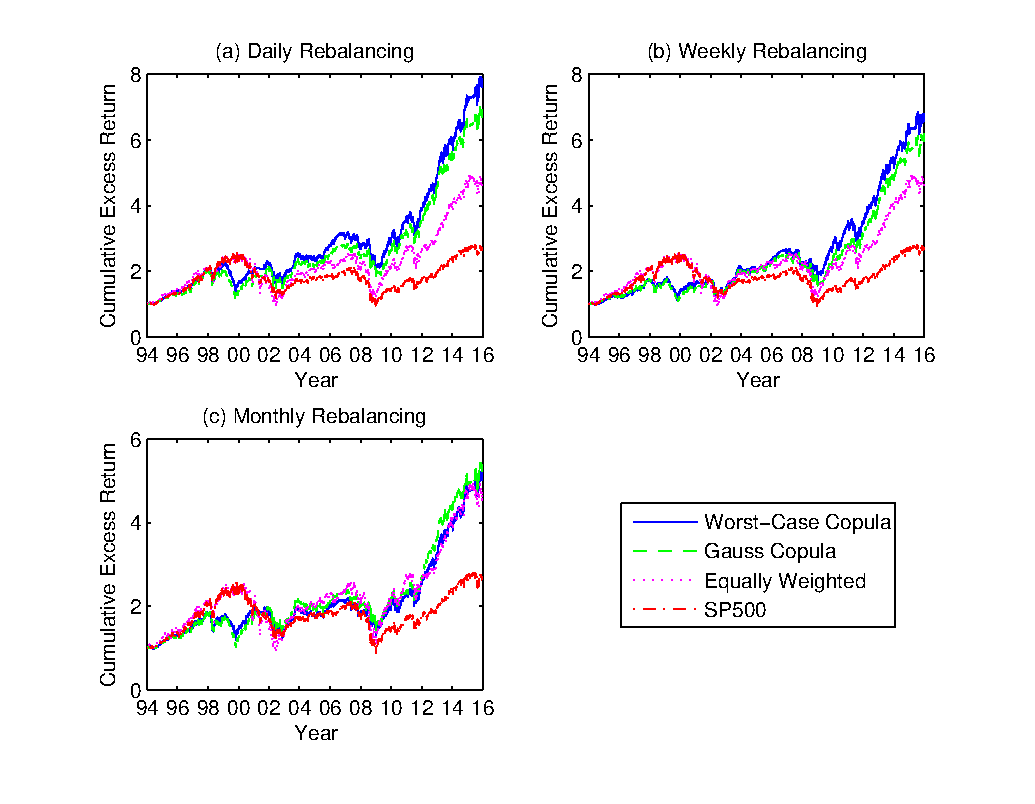
\includegraphics[scale=0.58]{fig1_nogrid.eps}
\caption{\scriptsize Cumulative excess returns of the portfolio strategies without daily target mean return }
\label{fig:fig01}
\end{figure}

\end{frame}

\begin{frame}[label=frame9d]
	\frametitle{Conclusions}
	
	\begin{itemize}
		\justifying
		
		\item By selecting a diversified set of assets over a long-term period we found that copula-based approaches offer better hedges against losses than the 1/N portfolio.
		
		\vspace{0.3cm}
		
		\item The WCCVaR approach generates portfolios with better downside
		risk statistics for any rebalancing period and it is more profitable than the Gaussian Copula-CVaR for daily and weekly rebalancing. 
		
		\end{itemize}
	
\end{frame}
		
		\begin{frame}[label=frame9e]
		\frametitle{Highlights}
		
		\begin{itemize}
			\justifying
		
		\item Worst-Case Copula Conditional Value-at-Risk Optimization using Lin-
		ear Programming
		
		\vspace{0.3cm}
		
		\item Risk management with high-dimensional copulas without pair-copula
		constructions
		
		\vspace{0.3cm}
		
		\item We select a diversified set of assets that can be useful during any market conditions
		
		\vspace{0.3cm}
		
		\item We compare the performance of Gaussian, Worst-Case and Equally
		Weighted portfolios
		
		\vspace{0.3cm}
		
		\item Copula-based models show a superior performance after the subprime
		mortage crisis
		
		\end{itemize}
	
\end{frame}


\begin{frame}

\centering
\Large{Thanks! Any questions?}

\end{frame}

\end{document}


